\documentclass{report}
\usepackage[left=20mm, top=15mm, right=20mm, bottom=15mm, nohead, nofoot]{geometry}
\usepackage[T2A]{fontenc}
\usepackage[utf8]{inputenc}
\usepackage[russian]{babel}
\usepackage{amsmath}
\usepackage{graphicx}
\graphicspath{{../}}
\DeclareGraphicsExtensions{.png}

\title{Решение уравнения Лапласа методом конечных элементов с помощью FEniCS}
\author{Шклярик Ю.Н., 6 группа, 3 курс}
\date{}

\begin{document}

\maketitle

\chapter{Решение задачи на прямоугольной области с разрывными граничными условиями Дирихле}

\section{Постановка задачи}
Рассчитать поле, порождаемое заряженной пластиной в однородной среде.

\section{Математическая модель}
\begin{equation}
	\begin{cases}
		\Delta u = 0, \\
		u(0, y) = 0,&u(a, y)=0,\\
		u(x, 0) = 0,&u(x, b)=f(x),
	\end{cases}
\end{equation}
где $f(x) = \alpha I_{[l,r]}(x)$.

\section{Аналитическое решение}
Воспользуемся методом разделения переменных. Будем искать решение в виде
\begin{equation*}
	u(x,y) = X(x)Y(y).
\end{equation*}
Получаем систему уравнений
\begin{equation}
	\frac{X''(x)}{X(x)}=-\frac{Y''(y)}{Y(y)}=-\lambda.
\end{equation}
Задача Штурма-Лиувилля для $X(x)$:
\begin{equation}\label{sl1}
	\begin{cases}
		X''(x)+\lambda X(x)=0,\\
		X(0)=X(a)=0.
	\end{cases}
\end{equation}

Получаем собственные значения:
\begin{equation*}
	\sqrt{\lambda_n}=\mu_n=\frac{\pi n}{a} .
\end{equation*}
Собственные функции для задачи (\ref{sl1}) с точностью до константы имеют вид
\begin{equation*}
	X_n(x)=\sin{\mu_n x}.
\end{equation*}
Задача для $Y(y)$:
\begin{equation}\label{sl2}
	\begin{cases}
		Y_n''(x)-\lambda_n Y_n(x)=0,\\
		Y_n(0)=0.
	\end{cases}
\end{equation}
Имеем
\begin{equation}
	Y_n(y)=C_{n_1}e^{-\mu_n  y}+C_{n_2}e^{\mu_n  y}
\end{equation}
\begin{equation*}
	Y_n(0)=C_{n_1} + C_{n_2} = 0.
\end{equation*}
Значит,
\begin{equation}
	Y_n(y)=C_n \sh{\mu_n y}
\end{equation}
\begin{equation}
	u(x,y) = \sum_{n=1}^{\infty}C_n \sh{\mu_n y} \sin{\mu_n x}
\end{equation}
\begin{equation*}
	C_n = \frac{2}{b sh{\mu_n b}}\int_0^b f(x) \sin{\mu_n x} dx = \frac{2\alpha}{b\sh{\mu_n b}}\int_l^r\sin{\mu_nx}dx =  \frac{2\alpha}{b\mu_n\sh{\mu_n b}}(\cos{\mu_n l} - \cos{\mu_n r})=
\end{equation*}
\begin{equation}
	=\frac{4\alpha}{b\mu_n\sh{\mu_n b}}\sin{\frac{\mu_n}{2}(l+r)}\sin{\frac{\mu_n}{2}(r-l)}.
\end{equation}
Окончательное решение:
\begin{equation}
	u(x,y)=\frac{4\alpha}{b}\sum_{n=1}^{\infty}\frac{\sin{\left(\frac{\mu_n}{2}(l+r)\right)}\sin{\left(\frac{\mu_n}{2}(r-l)\right)}}{\mu_n\sh{\mu_n b}}\sh{\mu_n y} \sin{\mu_n x}.
\end{equation}

\section{Решение методом конечных элементов}

\subsection{Слабая формулировка задачи}
Домножим уравнение $\Delta u = 0$ на пробную функцию $v$ и проинтегрируем по области $\Omega = (0,a)\times(0,b)$:
\begin{equation}
	\int_{\Omega}v \Delta u dx=0.
\end{equation}
По формуле интегрирования по частям,
\begin{equation}
	\int_{\Omega}v \Delta u dx=\int_{\partial \Omega}v\frac{\partial u}{\partial n}ds-\int_{\Omega}\nabla v\nabla u dx=-\int_{\Omega}\nabla v \nabla u dx.
\end{equation}
Слабая формулировка задачи:
\begin{equation}\label{weak_form}
	\int_{\Omega} \nabla v \nabla u dx=0
\end{equation}

\subsection{Визуализация}
Визуализация для случая $a=b=1$, $n=30$, $\alpha = 0.05$.
%\begin{center}
\begin{figure}[t]
	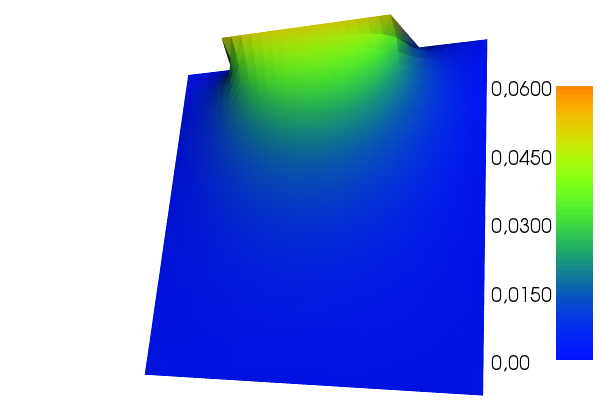
\includegraphics[scale=0.4]{dolfin_plot_0.png}
	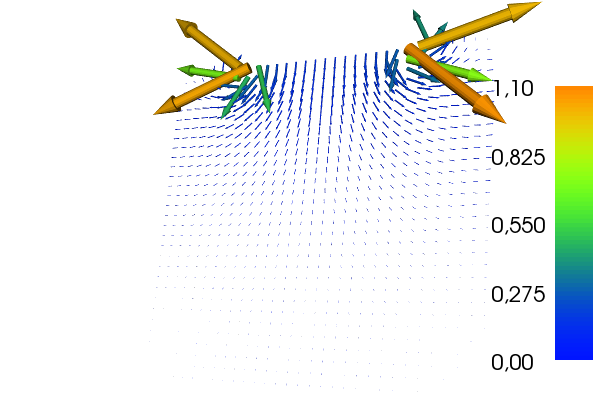
\includegraphics[scale=0.4]{dolfin_plot_1.png}
	\caption{Визуализация потенциала и напряжённости, полученных методом конечных элементов}
	\centering
%\end{center}
\end{figure}

\subsection{Оценка скорости сходимости численного решения}
Зададим шаг равномерной прямоугольной сетки $h=\frac{1}{n}$. Произведём эксперименты с $h_0>h_1>h_2>...$ и получим соответствующие невязки $e_0, e_1, e_2, ...$. Предположим, что $e_i=Ch_i^r$. По результатам 2-ух экспериментов можно оценить $r$:
\begin{equation}
	r = \frac{\ln{\frac{e_{i+1}}{e_i}}}{\ln{\frac{h_{i+1}}{h_i}}}.
\end{equation}
\begin{center}
Результат:\\
n=  8 e=0.00057016 r=-0.285764\\
n= 16 e=0.00069505 r=2.118793\\
n= 32 e=0.00016003 r=-0.557871\\
n= 64 e=0.00023558 r=2.017781\\
n=128 e=0.00005817 r=-0.613936\\
\end{center}

\chapter{Решение задачи на прямоугольной области с непрерывными граничными условиями Дирихле}
\section{Постановка задачи}
\begin{equation}\label{eq2}
	\begin{cases}
		\Delta u = 0, \\
		u(0, y) = 1-y^2,&u(1, y)=2-y^2,\\
		u(x, 0) = 1+x^2,&u(x, 1)=x^2,
	\end{cases}
\end{equation}

\section{Аналитическое решение}
Решением уравнения (\ref{eq2}) является функция
\begin{equation}
	u=1+x^2-y^2.
\end{equation}

\section{Решение методом конечных элементов}
\subsection{Визуализация}
\begin{figure}[h]
	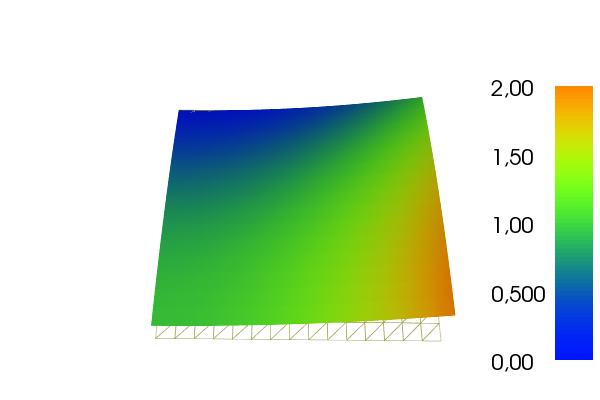
\includegraphics[scale=0.4]{dolfin_plot_5.png}
	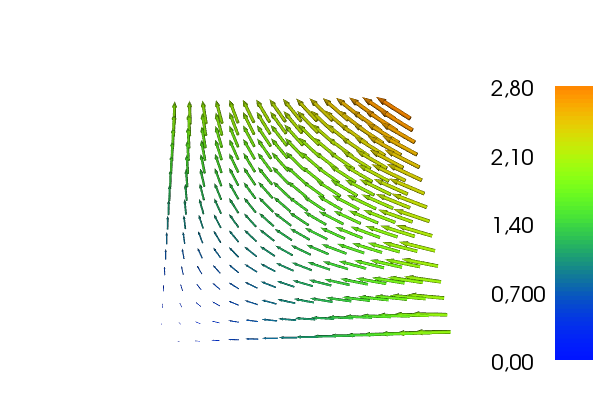
\includegraphics[scale=0.4]{dolfin_plot_4.png}
	\caption{Визуализация потенциала и напряжённости, полученных методом конечных элементов}
	\centering
\end{figure}

\subsection{Оценка скорости сходимости численного решения}
Зададим шаг равномерной прямоугольной сетки $h=\frac{1}{n}$. Произведём эксперименты с $h_0>h_1>h_2>...$ и получим соответствующие невязки $e_0, e_1, e_2, ...$. Предположим, что $e_i=Ch_i^r$. По результатам 2-ух экспериментов можно оценить $r$:
\begin{equation}
	r = \frac{\ln{\frac{e_{i+1}}{e_i}}}{\ln{\frac{h_{i+1}}{h_i}}}.
\end{equation}
Результат:\\
\begin{center}
n=~~4~e=0.00658808 ~r=1.999999999999993\\
n=~~8~ e=0.00164702~ r=1.999999999999982\\
n=~16 ~e=0.00041175~ r=1.999999999999973\\
n=~32 ~e=0.00010294~ r=1.999999999999943\\
n=~64 ~e=0.00002573~ r=1.999999999999871\\
n=128 ~e=0.00000643~ r=1.999999999999731\\
n=256 ~e=0.00000161
\end{center}
Можно сделать вывод, что погрешность метода имеет квадратичную зависимость от шага сетки.

\chapter{Решение задачи в цилиндрических координатах}
\section{Постановка задачи}
\begin{equation}
	\begin{cases}
		\Delta u = 0,\\
		u|_{r=a}=\cfrac{1}{a},\\
		u|_{r=b}=\cfrac{1}{b}.
	\end{cases}
\end{equation}

\section{Визуализация}
\begin{figure}[h]
	\centering
	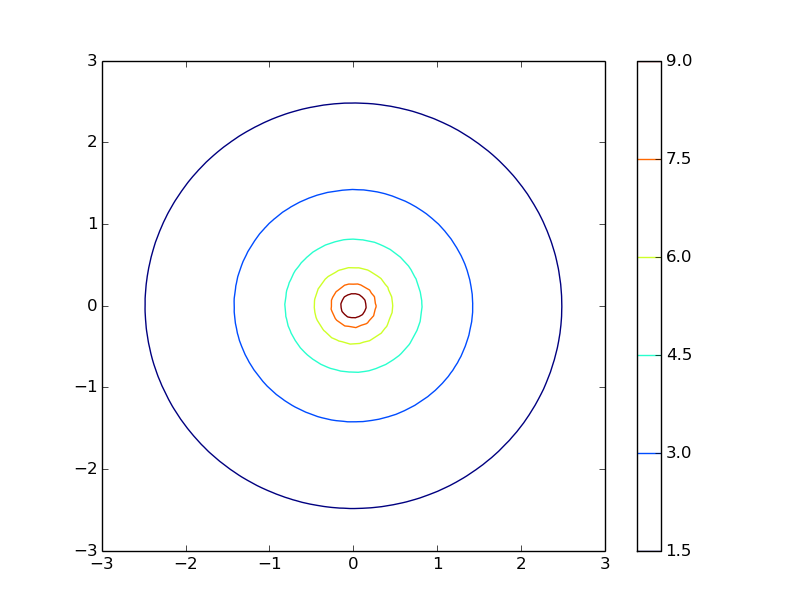
\includegraphics[scale=0.5]{contour.png}
	\caption{График изолиний}
\end{figure}

\section{Задача для тонкого диска}
\subsection{Постановка задачи}
\begin{equation}
	\begin{cases}
		\Delta u = 0,\\
		\cfrac{\partial u}{\partial z}\Bigr|_{z=0}=!!!,\\
		!!!
	\end{cases}
\end{equation}
\subsection{Слабая формулировка задачи}
Заменим условие на бесконечности условием на достаточно большом радиусе, так как заряженный диск можно считать точечным зарядом на больших расстояниях.

Также, воспользуемся осевой симметрией и сведём трёхмерную задачу на цилиндре к двумерной задаче на прямоугольнике переходом от декартовых координат к цилиндрическим.

Оператор Лапласа в цилиндрических координатах:
\begin{equation}
	\Delta u = \cfrac{1}{\rho}\cfrac{\partial}{\partial \rho}\left(\rho\cfrac{\partial u}{\partial \rho}\right) + \cfrac{1}{\rho^2}\cfrac{\partial^2u}{\partial \varphi^2}+\cfrac{\partial^2u}{\partial z^2}.
\end{equation}

Домножим уравнение $\Delta u = 0$ на пробную функцию $v$ и проинтегрируем по области $\Omega = (0,R)\times(0,h)$ и рассмотрим левую часть:
\begin{equation*}
\int\limits_{\Omega_{X}} \Delta_{(x,y,z)} u v d\Omega_{X} = \int\limits_{\Omega} \left( \cfrac{\partial u}{\partial \rho}v + \cfrac{\partial^2u}{\partial \rho^2}v\rho + \cfrac{\partial^2u}{\partial z^2}v\rho \right) d\Omega = \int\limits_{\Omega} \left( \cfrac{\partial u}{\partial \rho}v + \Delta u v\rho \right) d\Omega
\end{equation*}

\end{document}

